\documentclass[12pt,a4paper]{article}

% Packages
\usepackage{
    amsmath,
    amssymb,
    graphicx,
    titletoc,
    fancyhdr,
    geometry,
    babel,
    xcolor,
    enumerate,
    fix-cm,
    tocbibind,
    listings,
    float,
    enumitem,
    subcaption,
    hyperref
}

% Define colors
\definecolor{vgreen}{RGB}{104,180,104}
\definecolor{vblue}{RGB}{49,49,255}
\definecolor{vorange}{RGB}{255,143,102}

% Listings customization
\renewcommand\lstlistingname{Figura}
\renewcommand\lstlistlistingname{Figura}

\makeatletter
\newcommand*\@lbracket{[}
\newcommand*\@rbracket{]}
\newcommand*\@colon{:}
\newcommand*\colorIndex{%
    \edef\@temp{\the\lst@token}%
    \ifx\@temp\@lbracket \color{black}%
    \else\ifx\@temp\@rbracket \color{black}%
    \else\ifx\@temp\@colon \color{black}%
    \else \color{vorange}%
    \fi\fi\fi
}
\makeatother

% Setup for listings
\lstset{
    captionpos=b,
    belowcaptionskip=\bigskipamount,
    frame=single,
    basicstyle=\small\ttfamily,
    numbers=left,
    numberstyle=\tiny\color{gray},
    xleftmargin=2em,
    framexleftmargin=2em,
    backgroundcolor=\color{vgreen!10},
    stepnumber=1,
    showstringspaces=false,
    keywordstyle=\color{vblue},
    commentstyle=\color{gray},
    stringstyle=\color{vorange},
}

\begin{document}

\begin{titlepage}
    \centering
    
\includegraphics[scale=1]{M2_Modelos_de_Programación/reporte/figuras/Logo_Tec.png}\\
    \vspace{.5cm}
    \bfseries\large Escuela de Ingeniería y Ciencias
        
    \vspace{5cm}
    \centering
    \textbf{\Huge Cómputo en la Nube}
    \vspace{0.5cm}
        
    {\Large Creación de una Máquina Virtual de manera Local}

    \vspace{5cm}
        
    \textbf{\LARGE Armando Bringas Corpus}
        
    \vspace{0.5cm}
        
    {\large A01200230}
        
    \vfill
        
\end{titlepage}

\section{Introducción}

La siguiente práctica tiene como objetivo la implementación de una máquina virtual que nos permita tener entornos diferentes, en este caso en particular un sistema operativo diferente al de la computadora donde se estará virtualizando un sistema operativo Linux el cual tendrá un servidor web. Esto nos permitirá poder analizar las ventajas y desventajas de aplicaciones en la nube sobre una infraestructura local.

\section{Instalación de Oracle Virtual PC}

El primer paso es la instalación de Oracle VirtualBox el cual nos permitirá el generar diferentes entornos donde podrmos ejecutar diversos sistemas operativos en una mista computadora.

\begin{figure}[H]
    \centering
    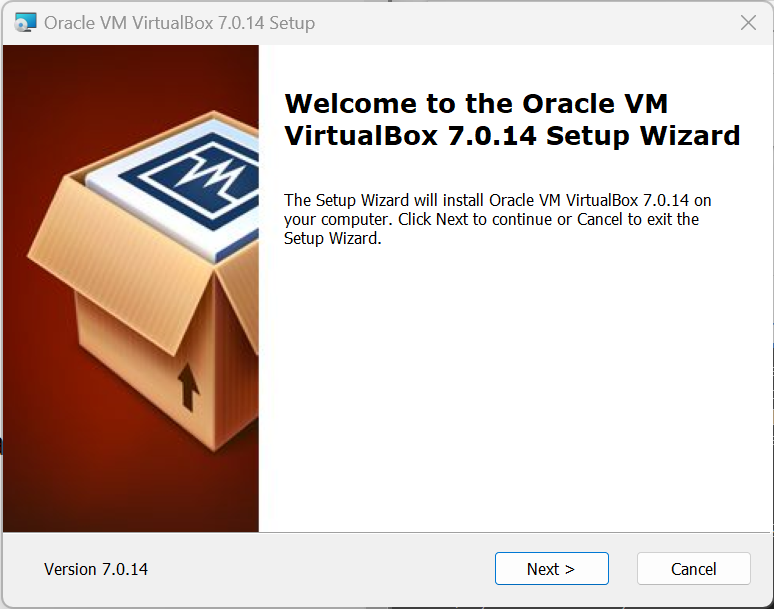
\includegraphics[width=1\linewidth]{M3_Virtualización_y_Contenedores/Tarea_2_Máquina_Virtual_Local/reporte/figuras/2-1_Instalación_Oracle_VM.png}
    \captionof{lstlisting}{Instalación de VirtualBox 7.0.14}
    \label{fig:Instalación_VirtualBox_1}
\end{figure}


\begin{figure}[H]
    \centering
    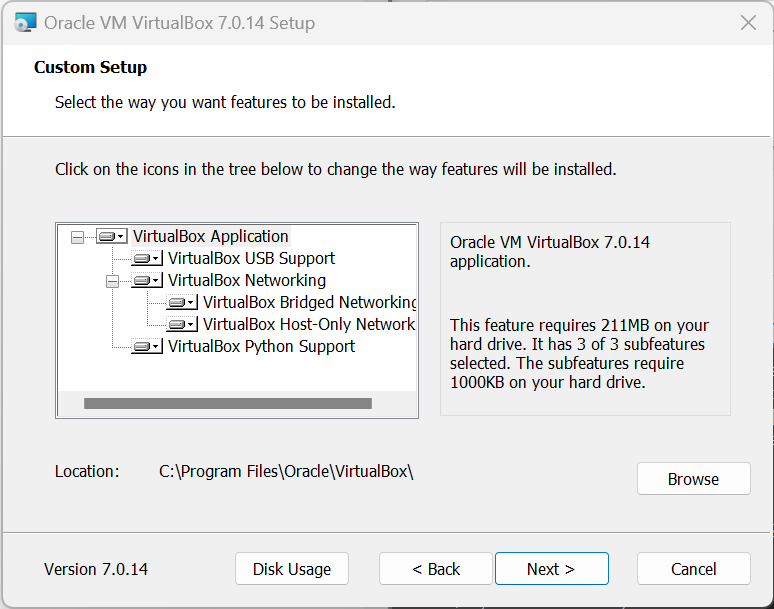
\includegraphics[width=1\linewidth]{M3_Virtualización_y_Contenedores/Tarea_2_Máquina_Virtual_Local/reporte/figuras/2-2_Instalación_Oracle_VM.png}
    \captionof{lstlisting}{Instalación de VirtualBox 7.0.14}
    \label{fig:Instalación_VirtualBox_2}
\end{figure}


\section{Creación de la Máquina Virtual de Debian}

El siguiente paso es la creación de una Máquina Virtual donde montaremos un pequeño servidor web quen estará basado en una distribución de Linux llamada Debian. Las siguientes imágenes muestran parte del proceso de instalación de Debian en la Máquina Virtual. Como configuraciones importantes para la creación de la Máquina Virtual enlistamos las siguientes:

\begin{itemize}
    \item Nombre: MVDebianLinuxWebServer
    \item Tipo (Sitema Operativo): Linuzx
    \item Versión: Debian (64-bit)
    \item Tamaño de memoria RAM: 1024 MB
    \item Disco duro: Disco Virtual (VDI - VirtualBox Disk Image) de 5GB con Reservado Dinámico para permitir su expansión
\end{itemizehttps://www.overleaf.com/project/65af392690627fc92d487f82}

Las siguientes imágenes \ref{fig:Instalación_Debian_1}, \ref{fig:Instalación_Debian_2}, son algunas capturas de pantalla que muestran la instalación de Debian a través de una interfaz gráfica (GUI) donde se realizaron diferentes configuraciones como el lenguaje, la zona horaria y localización del sistema, la configuración del servidor y cuentas, gestor de arranque (en este caso GRUB), la partición del disco e instalación de los paquetes.

\begin{figure}[H]
    \centering
    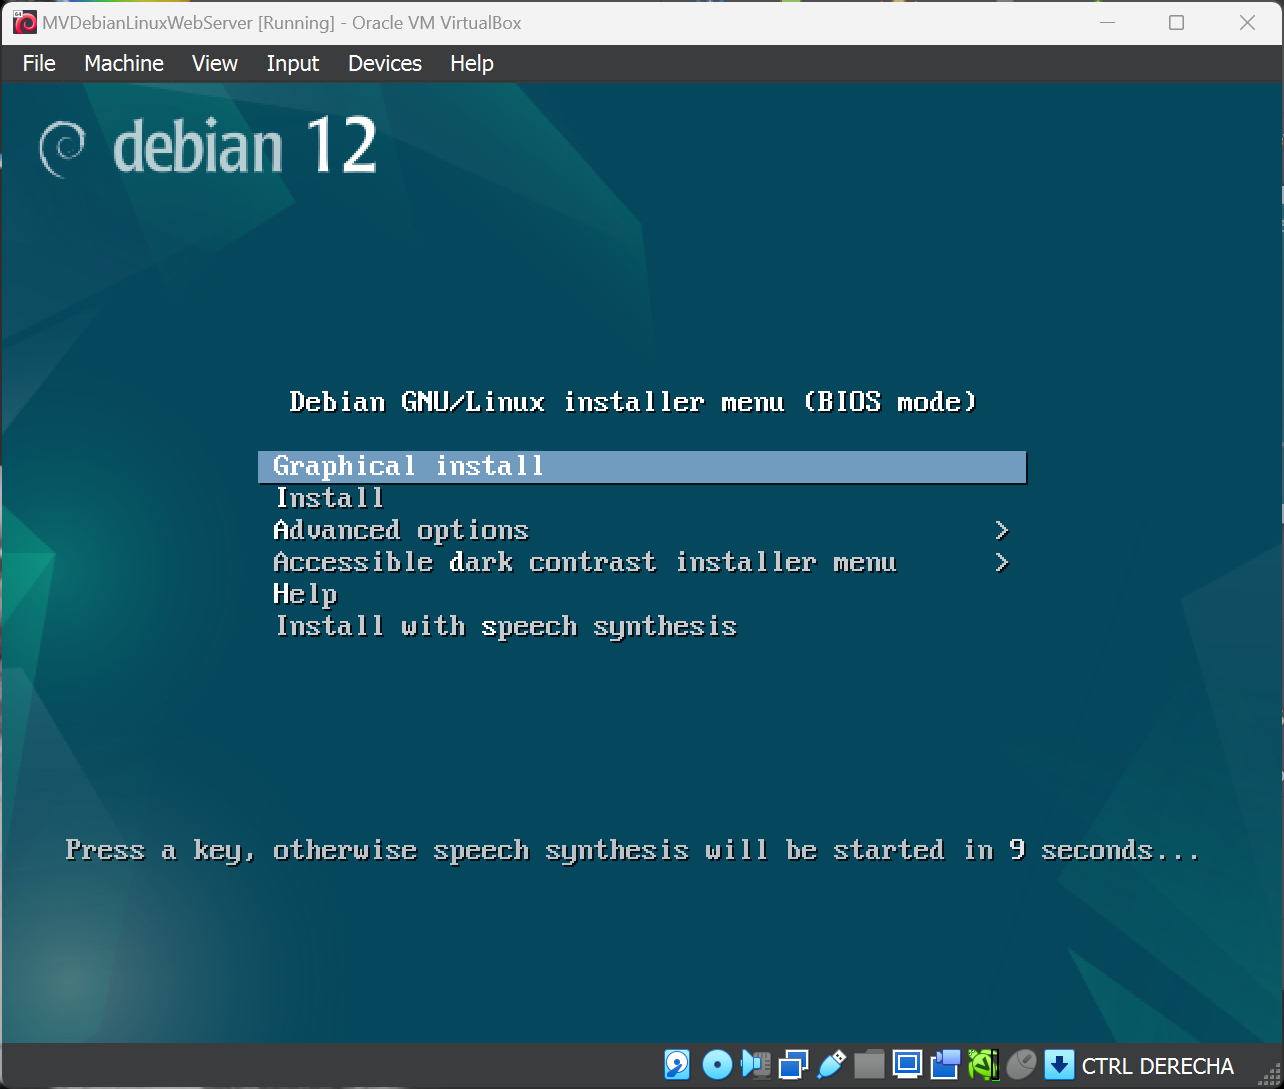
\includegraphics[width=1\linewidth]{M3_Virtualización_y_Contenedores/Tarea_2_Máquina_Virtual_Local/reporte/figuras/3-1_Máquina_Virtual_de_Debian.png}
    \captionof{lstlisting}{Instalación de Debian 12}
    \label{fig:Instalación_Debian_1}
\end{figure}


\begin{figure}[H]
    \centering
    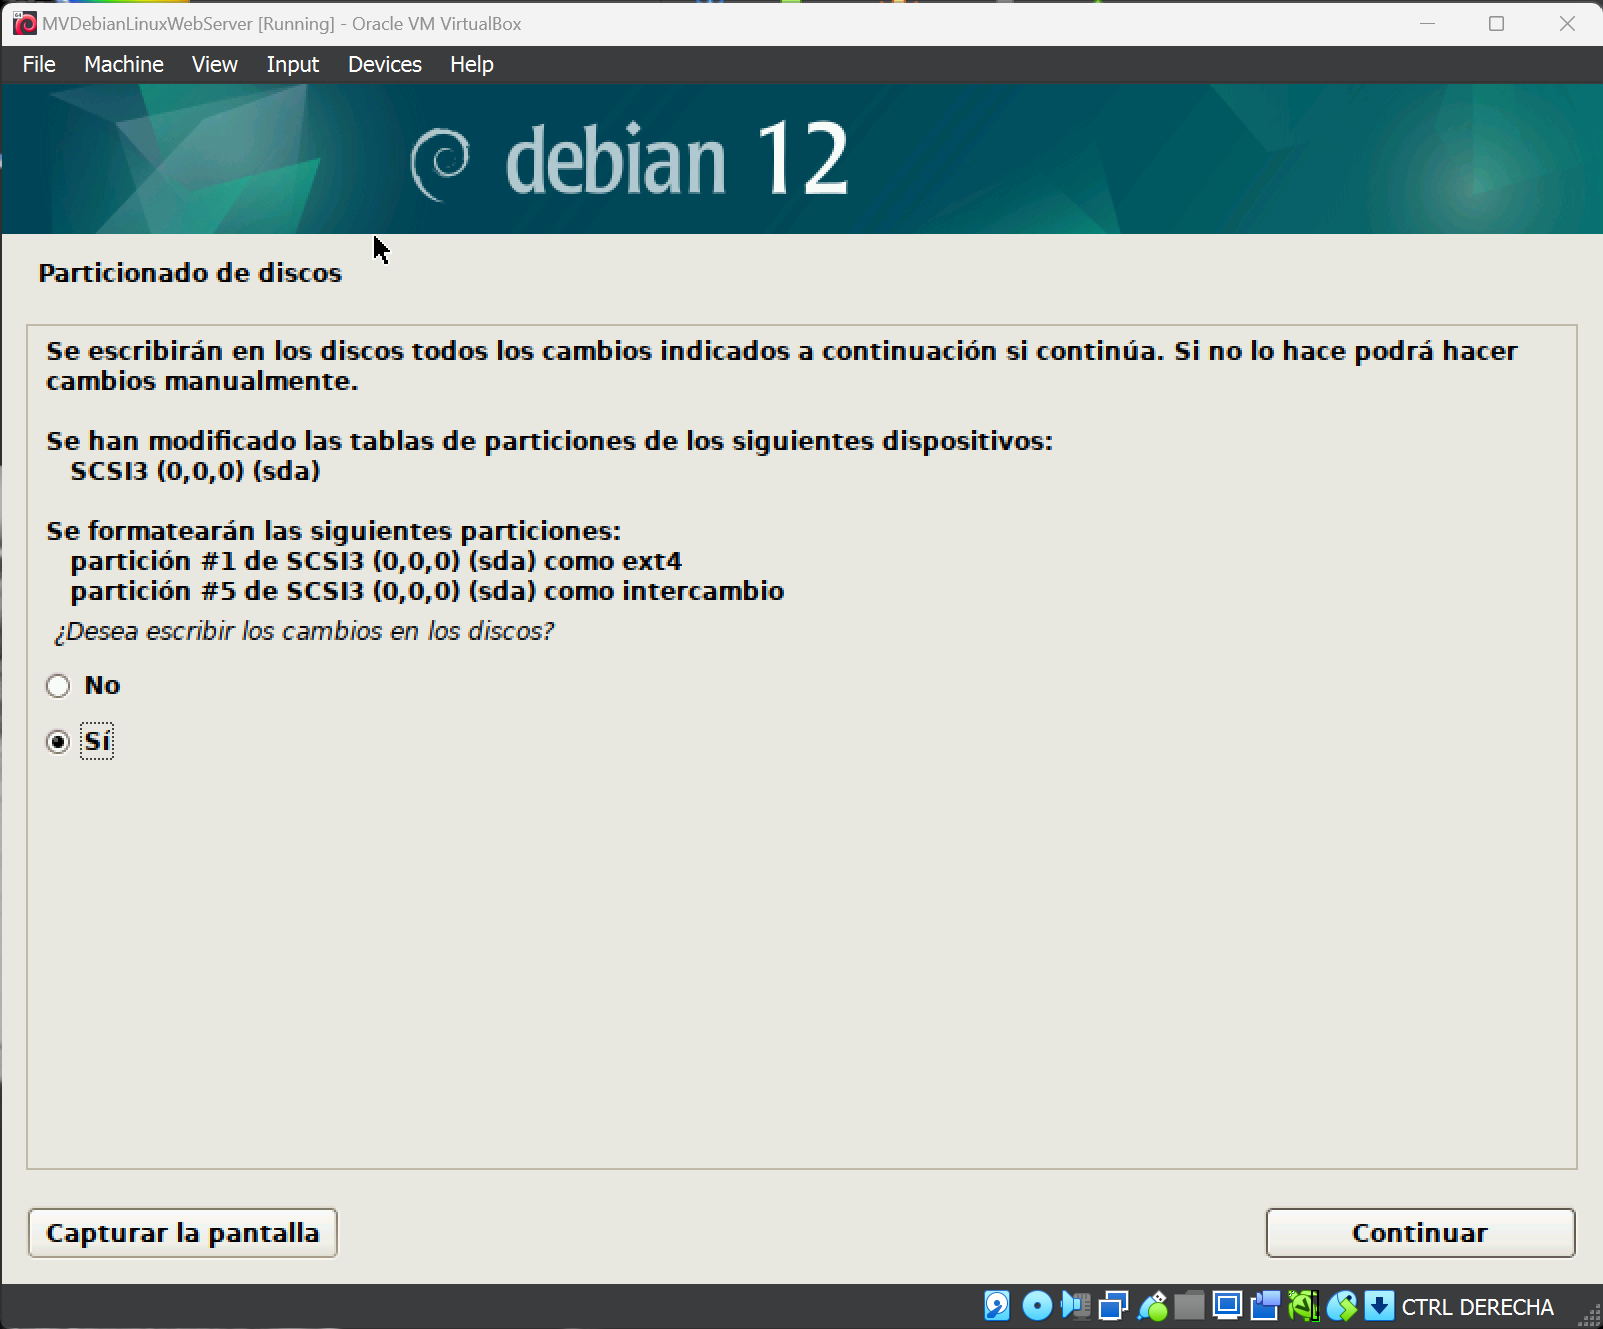
\includegraphics[width=1\linewidth]{M3_Virtualización_y_Contenedores/Tarea_2_Máquina_Virtual_Local/reporte/figuras/3-2_Máquina_Virtual_de_Debian.png}
    \captionof{lstlisting}{Instalación de Debian 12}
    \label{fig:Instalación_Debian_2}
\end{figure}

\vspace{1em}

Posteriormente, como se muestra en la imagen \ref{fig:Instalación_Debian_3} arrancamos el sistema, el gestor de arranque GRUB automáticamente inicia nuestro sistema operativo Debian y una vez cargado para poder trabajar con el, se ingresa el usuario raíz y la contraseña.

\begin{figure}[H]
    \centering
    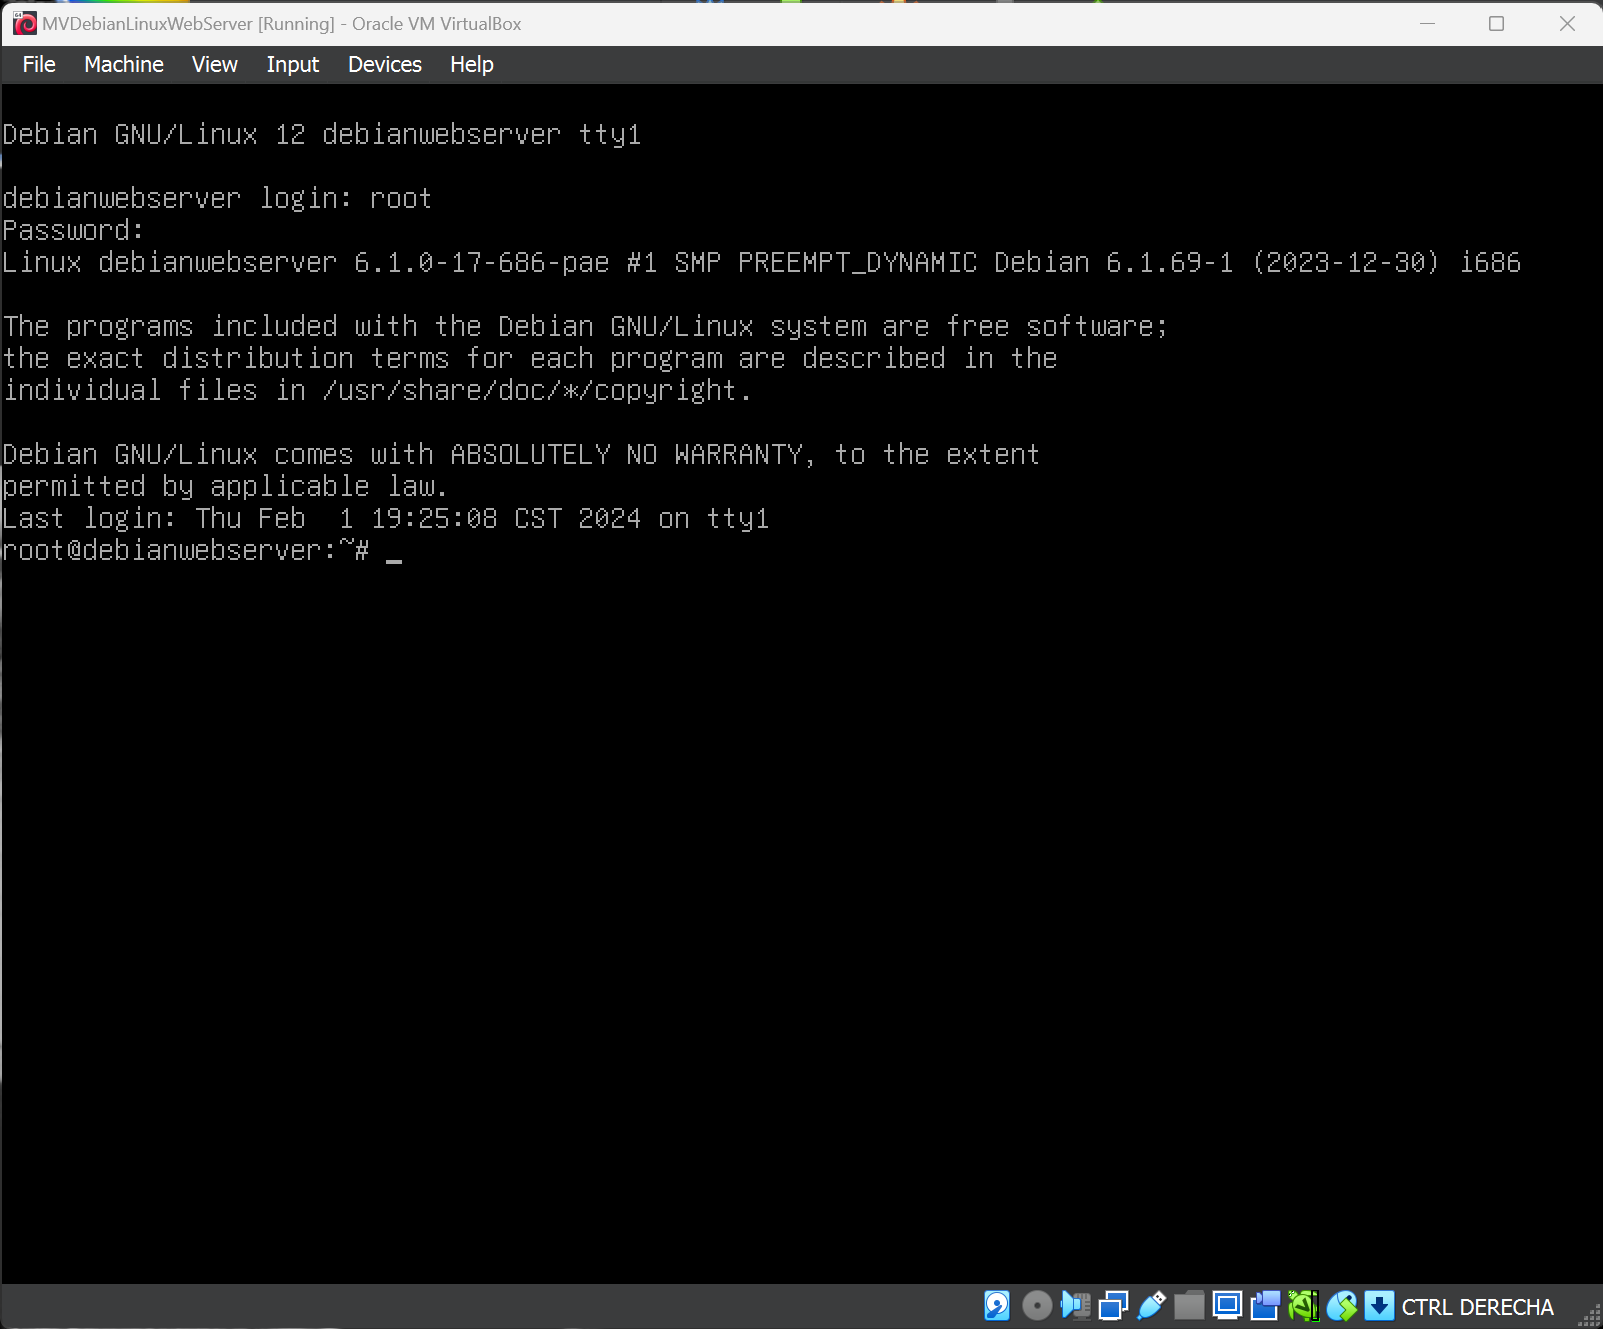
\includegraphics[width=1\linewidth]{M3_Virtualización_y_Contenedores/Tarea_2_Máquina_Virtual_Local/reporte/figuras/3-3_Máquina_Virtual_de_Debian.png}
    \captionof{lstlisting}{Instalación de Debian 12}
    \label{fig:Instalación_Debian_3}
\end{figure}


\section{Instalación y configuración de los servicios}

Una vez que accedemos al sistema operativo de nuestra máquina virtual se procede a instalar los paquetes que nos permitirán conocer la IP de la Máquina Virtual, en este caso por medio de comando \textbf{apt install net-tools}. La imagen \ref{fig:Configuración_serivicios_1} muestra que los paquetes solicitados ya están instalados con su versión más reciente, esto es debido que previamente a la toma de captura ya se había ejecutado el comando.


\begin{figure}[H]
    \centering
    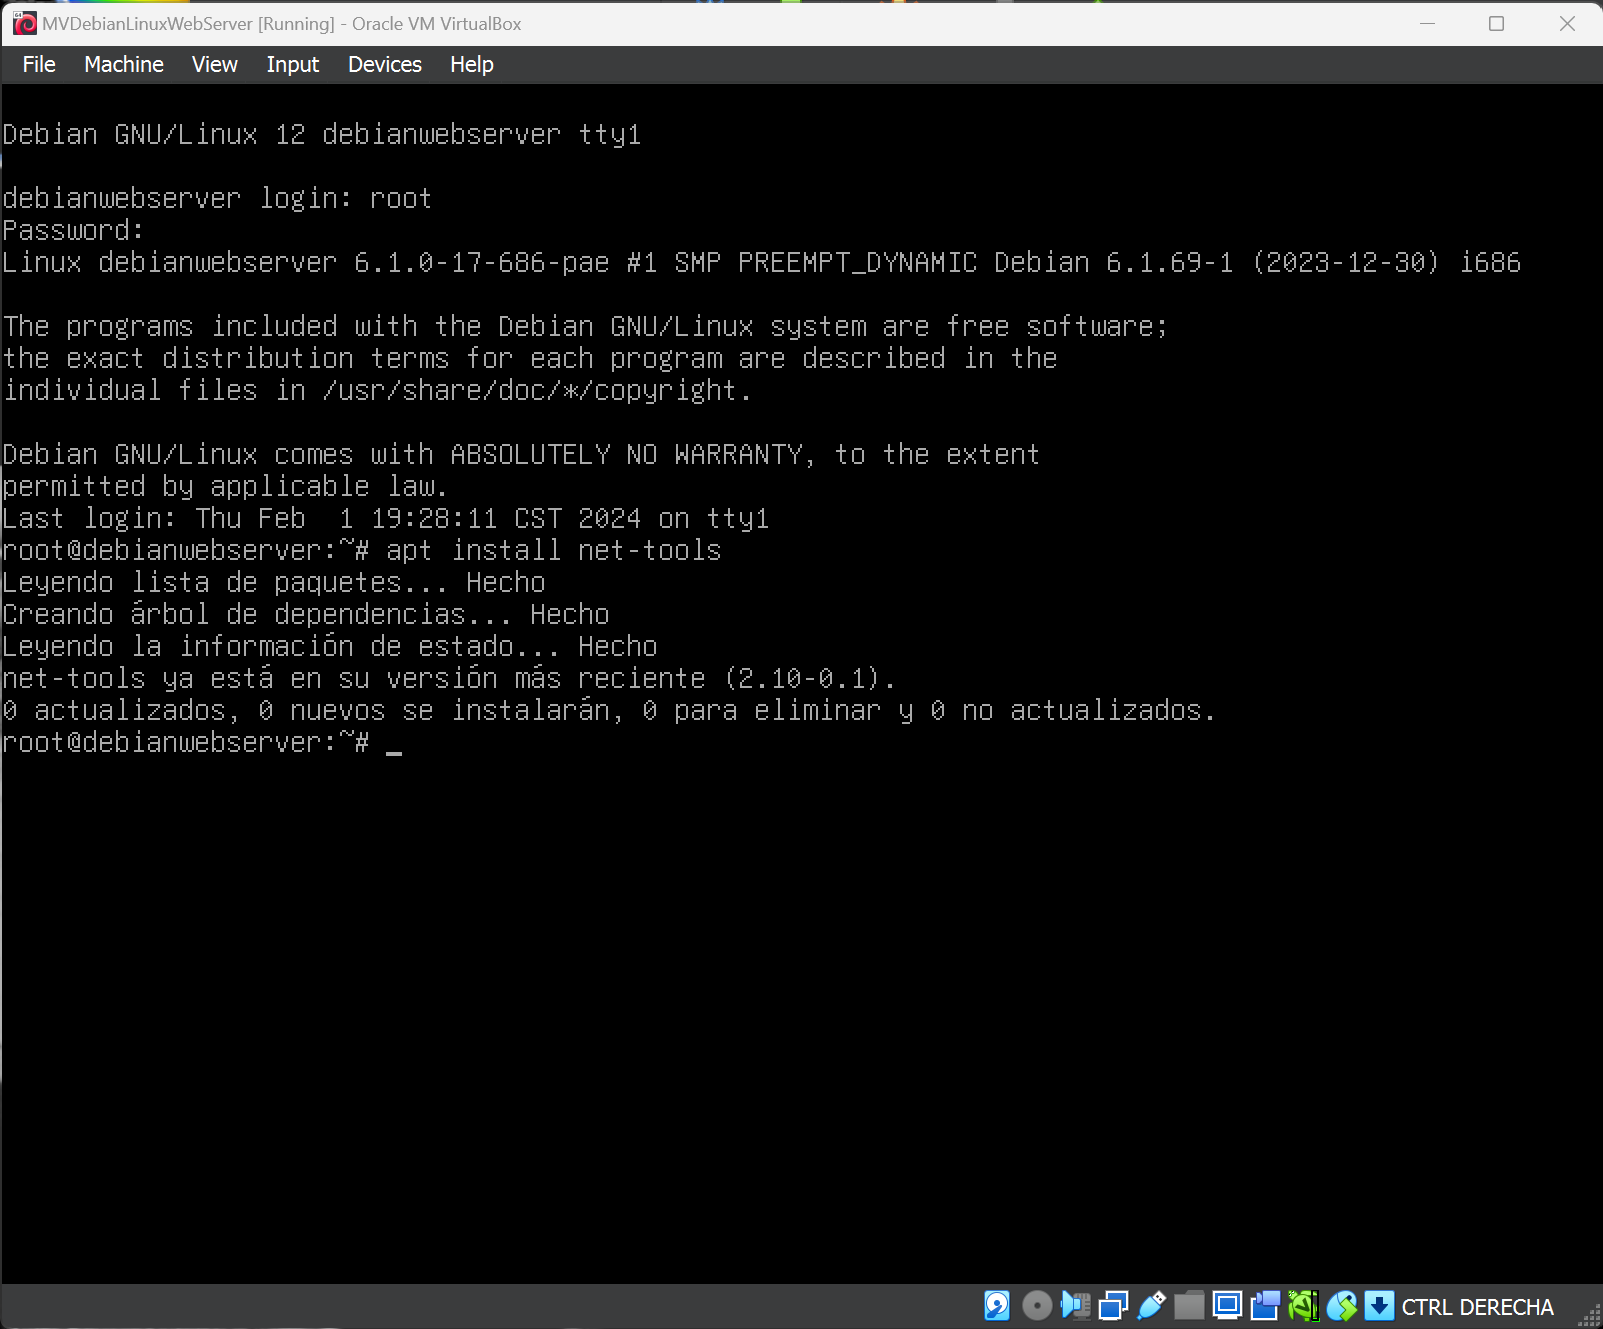
\includegraphics[width=1\linewidth]{M3_Virtualización_y_Contenedores/Tarea_2_Máquina_Virtual_Local/reporte/figuras/4-1_Configuración_servicios.png}
    \captionof{lstlisting}{Configuración de los Servicios}
    \label{fig:Configuración_serivicios_1}
\end{figure}


A través del comando \textbf{ifconfig -a} podemos desplegar la configuración de la red del sistema operativo que se encuentra ejecutando la Máquina Virtual como se observa en la figura \ref{fig:Configuración_serivicios_2}, en donde más adelante ocuparemos la dirección IP para poder acceder al pequeño servidor que se estará levantando


\begin{figure}[H]
    \centering
    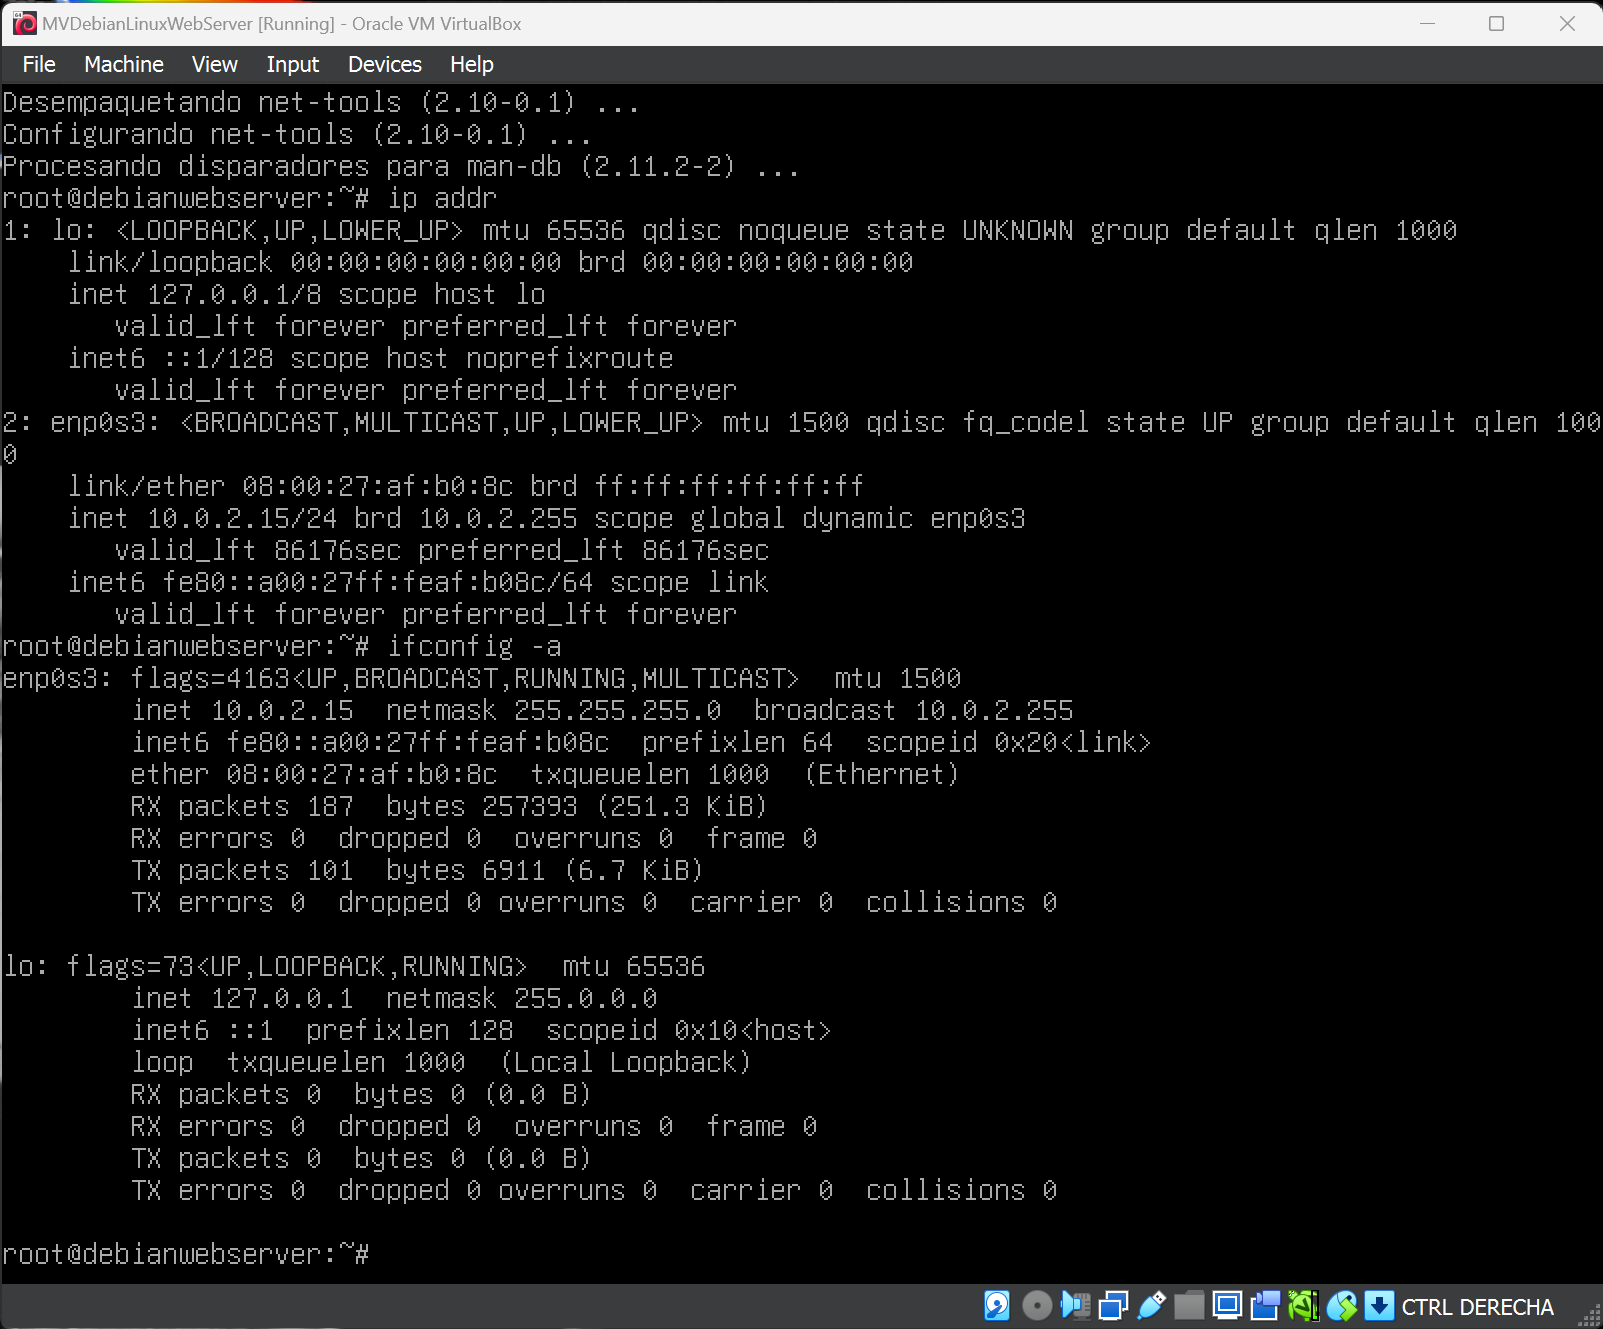
\includegraphics[width=1\linewidth]{M3_Virtualización_y_Contenedores/Tarea_2_Máquina_Virtual_Local/reporte/figuras/4-2_Configuración_servicios.png}
    \captionof{lstlisting}{Configuración de los Servicios}
    \label{fig:Configuración_serivicios_2}
\end{figure}


\section{Personalización del sitio web}


Descargamos la plantilla web del siguiente sitio \url{ https://htmltemplates.co/free-website-templates/minimal-personal-portfolio-free-portfolio-html-template} y procedemos a realizar algunas modificaciones y personalizaciones, este caso utilizamos Visual Studio Code como se muestra en la figura \ref{fig:Personalización_sitio_web_1}. En la figura \ref{fig:Personalización_web_2} se pueden observar las modificaciones que estuvimos realizando como por ejemplo en el color de fondo, la imagen, descripción, etc. 

Las modificaciones realizadas se pueden consultar en el siguiente repositorio de Github:
\url{https://github.com/armandoBringas/Cloud_Computing/tree/main/M3_Virtualizaci%C3%B3n_y_Contenedores}


\begin{figure}[H]
    \centering
    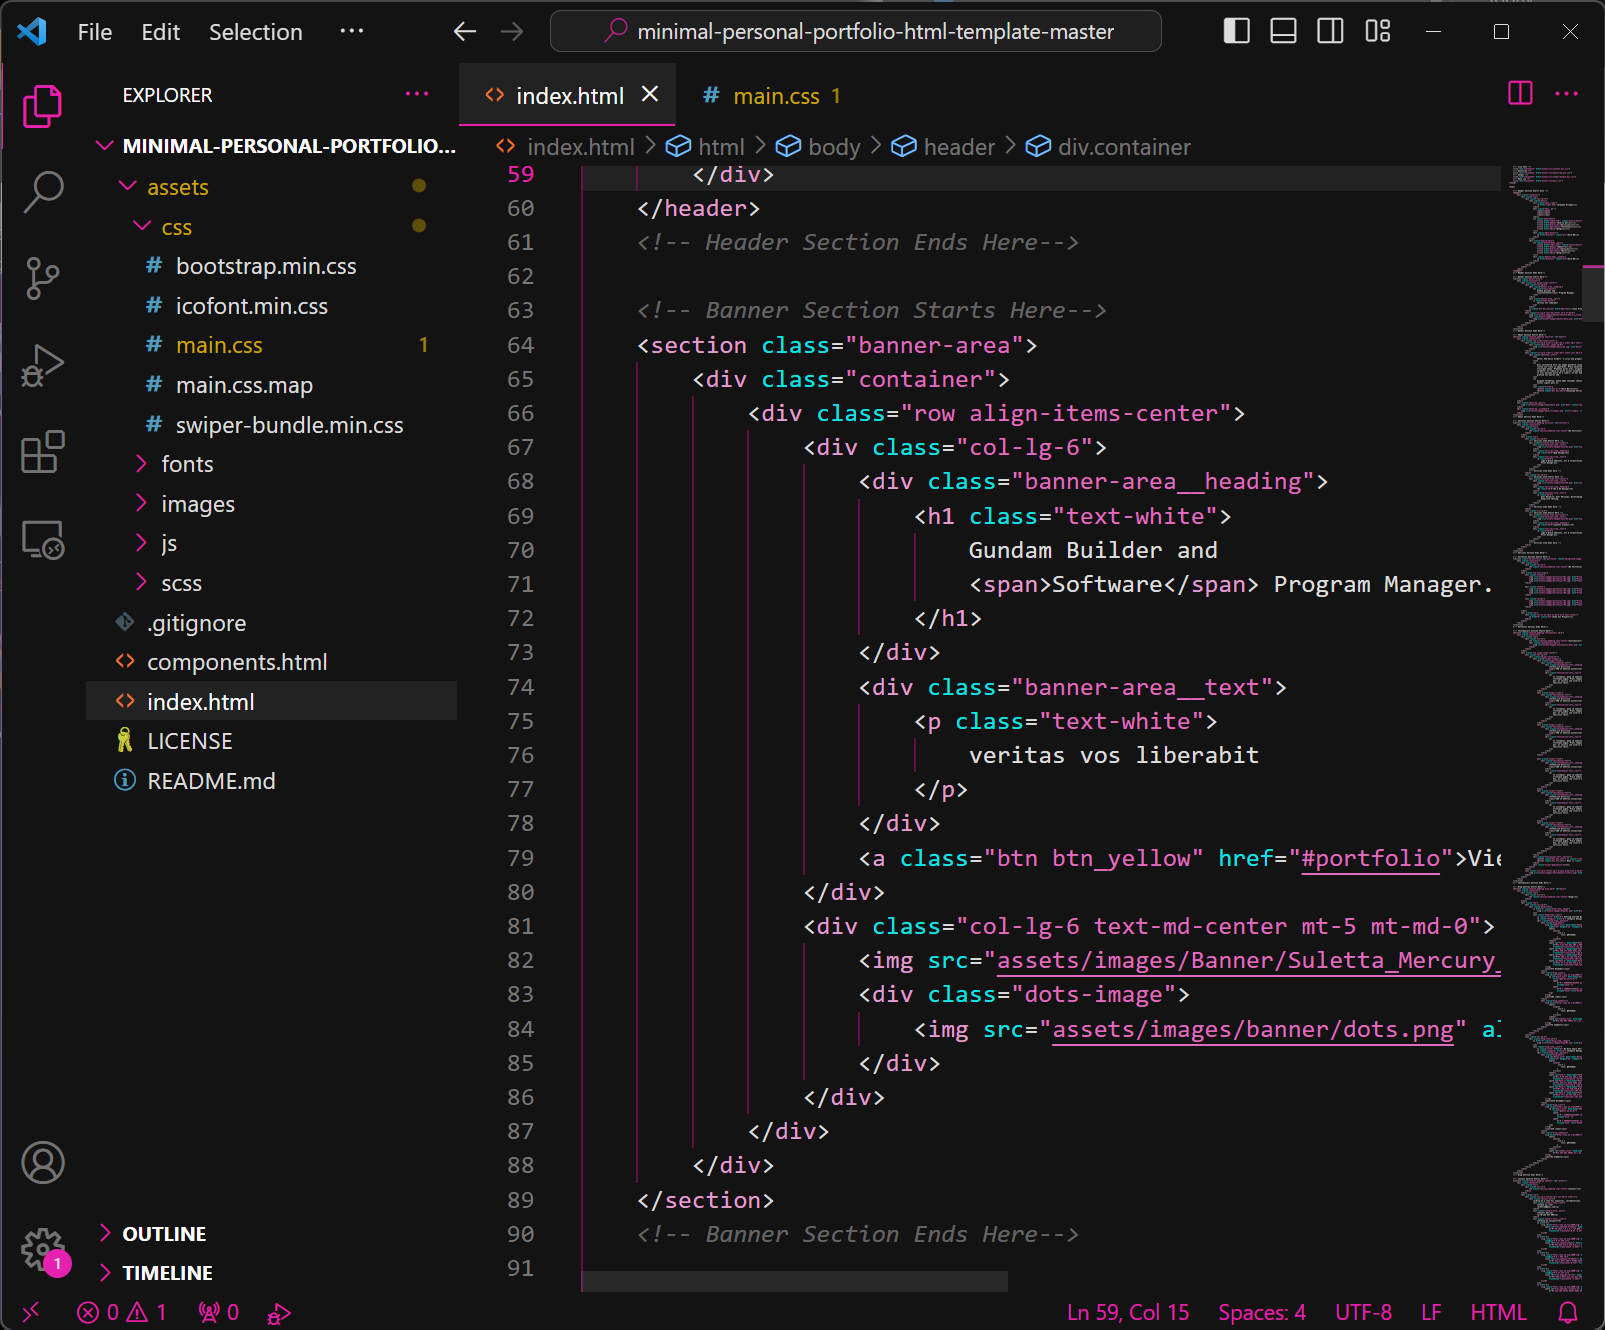
\includegraphics[width=.75\linewidth]{M3_Virtualización_y_Contenedores/Tarea_2_Máquina_Virtual_Local/reporte/figuras/5-1_Personalización_Sitio_Web.png}
    \captionof{lstlisting}{Personalización del Sitio Web}
    \label{fig:Personalización_sitio_web_1}
\end{figure}

\begin{figure}[H]
    \centering
    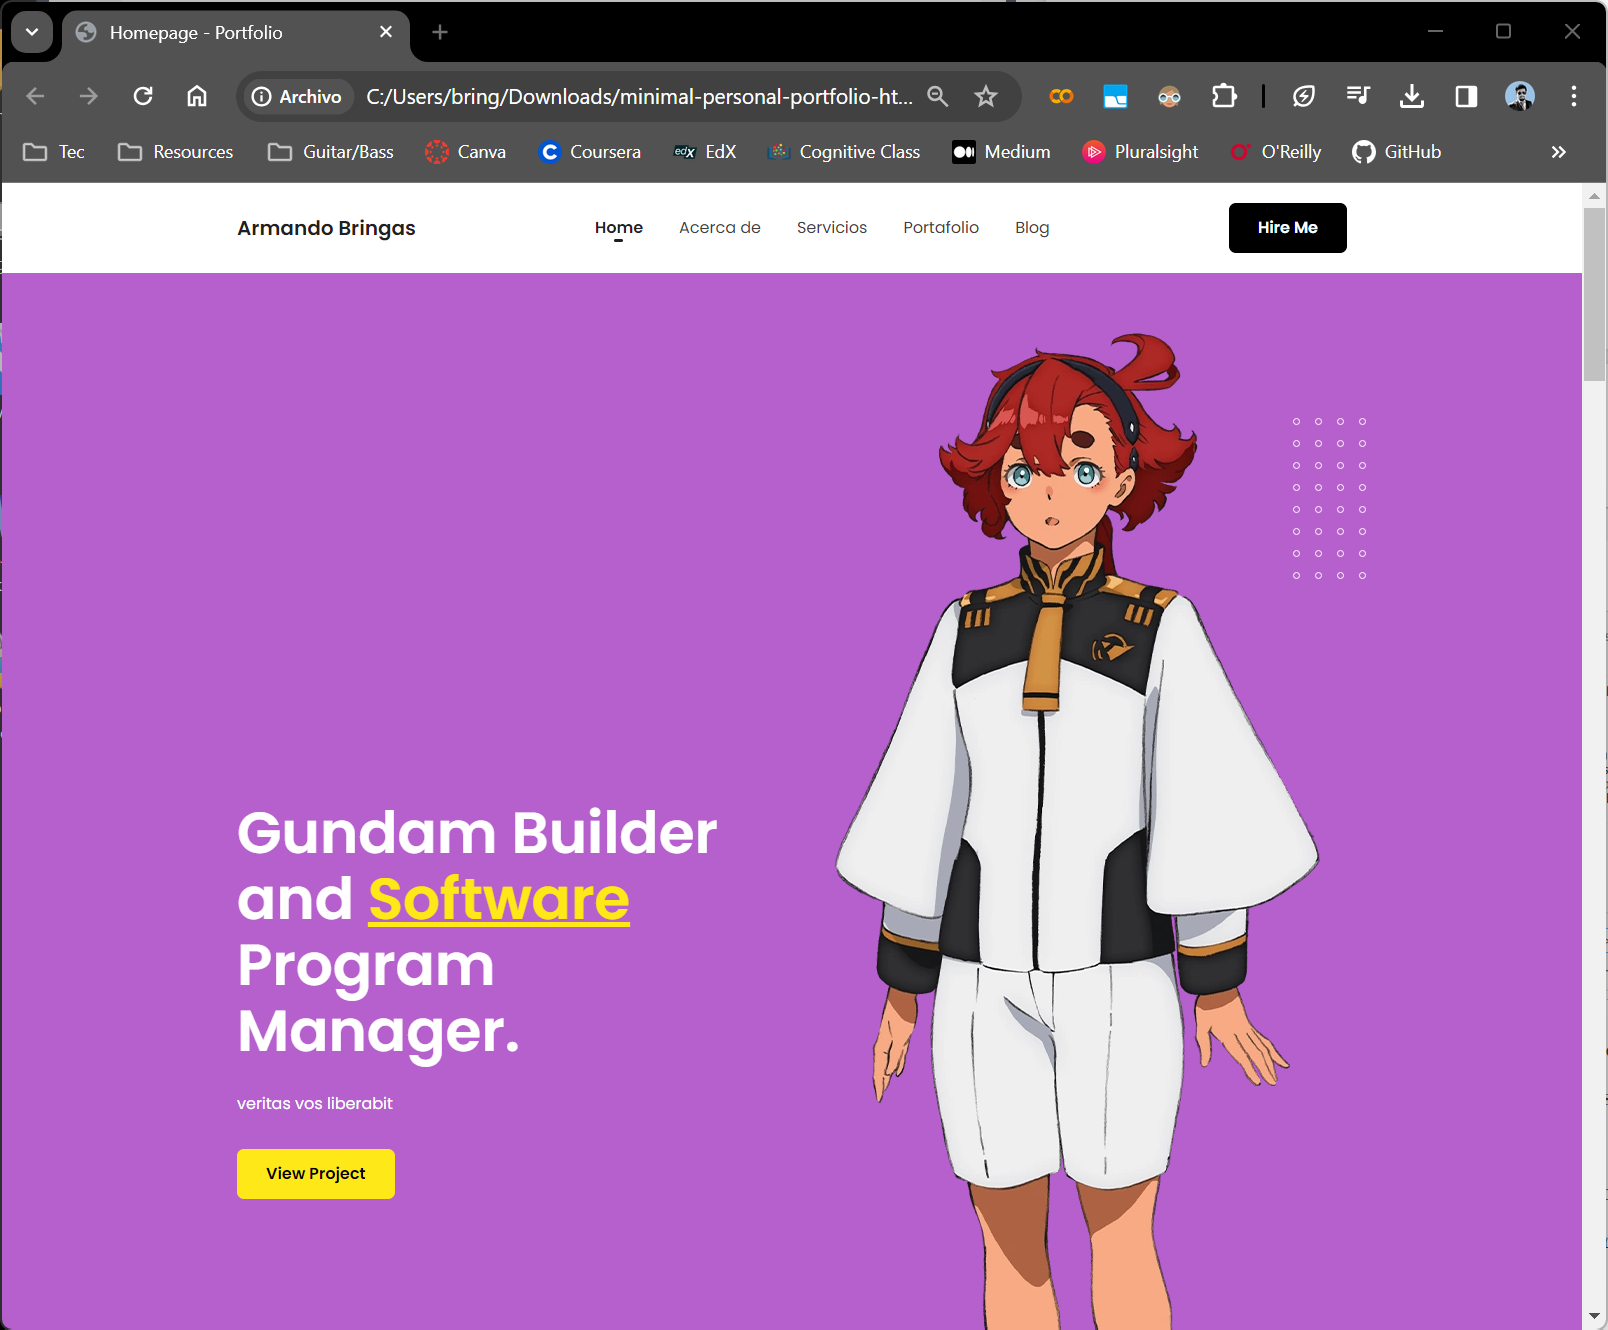
\includegraphics[width=.75\linewidth]{M3_Virtualización_y_Contenedores/Tarea_2_Máquina_Virtual_Local/reporte/figuras/5-2_Personalización_Sitio_Web.png}
    \captionof{lstlisting}{Personalización del Sitio Web}
    \label{fig:Personalización_sitio_web_2}
\end{figure}


\section{Carga de Sitio Web en la Máquina Virtual}

Posteriormente cargamos nuestro sitio web a la Máquina Virtual, para este caso utilizamos un gestor de archivos para sitios remotos llamado FileZilla, en donde primeramente en VirtualBox habilitamos el permitir la conexión entre nuestra computadora y la máquina virtual. La figura \ref{fig:Cargado_sitio_web_1} muestra la configuración para establecer la conexión y realizar la transferencia de archivos entre la computadora y la Máquina Virtual.

\begin{figure}[H]
    \centering
    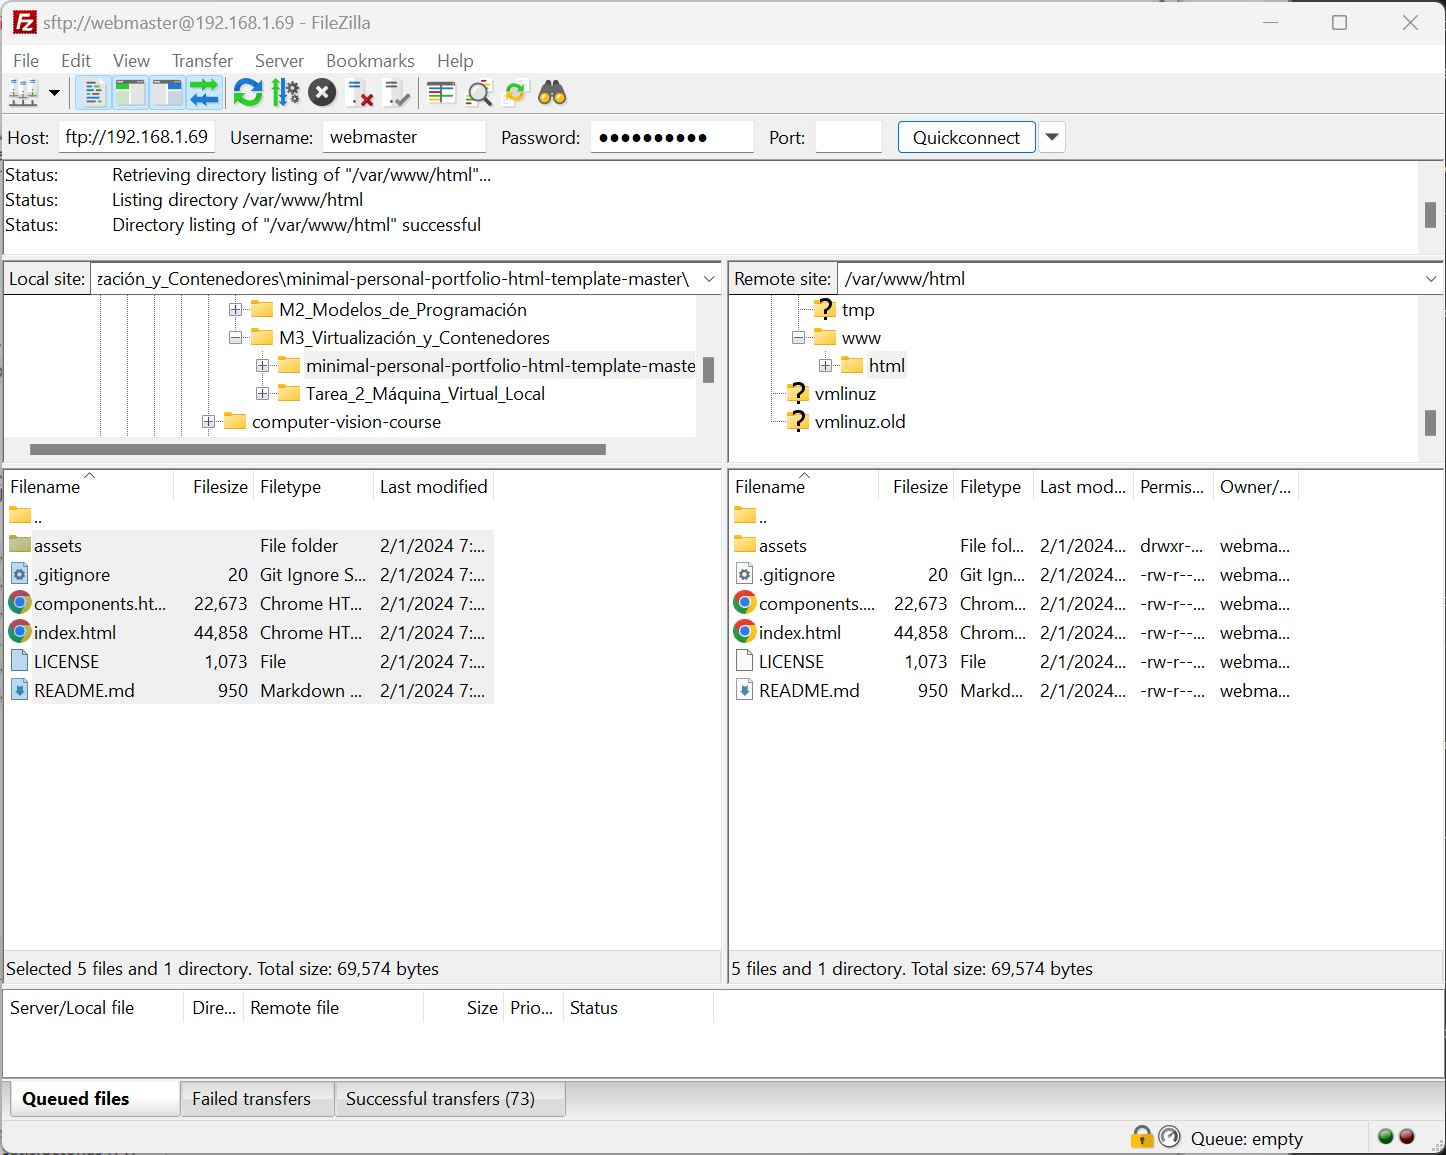
\includegraphics[width=1\linewidth]{M3_Virtualización_y_Contenedores/Tarea_2_Máquina_Virtual_Local/reporte/figuras/6-1_Carga_Sitio_Web_en_MV.png}
    \captionof{lstlisting}{Cargado de sitio web en la Máquina Virtual}
    \label{fig:Cargado_sitio_web_1}
\end{figure}

Finalmente ejecutamos nuestra Máquina Virtual con nuestro usuario raíz y ejecutamos el comando \textbf{chmod 777 html/} para poder escribir en el directorio html y así poder copiar a través de FileZilla los archivos en el sitio remoto de la Máquina Virtual.

\begin{figure}[H]
    \centering
    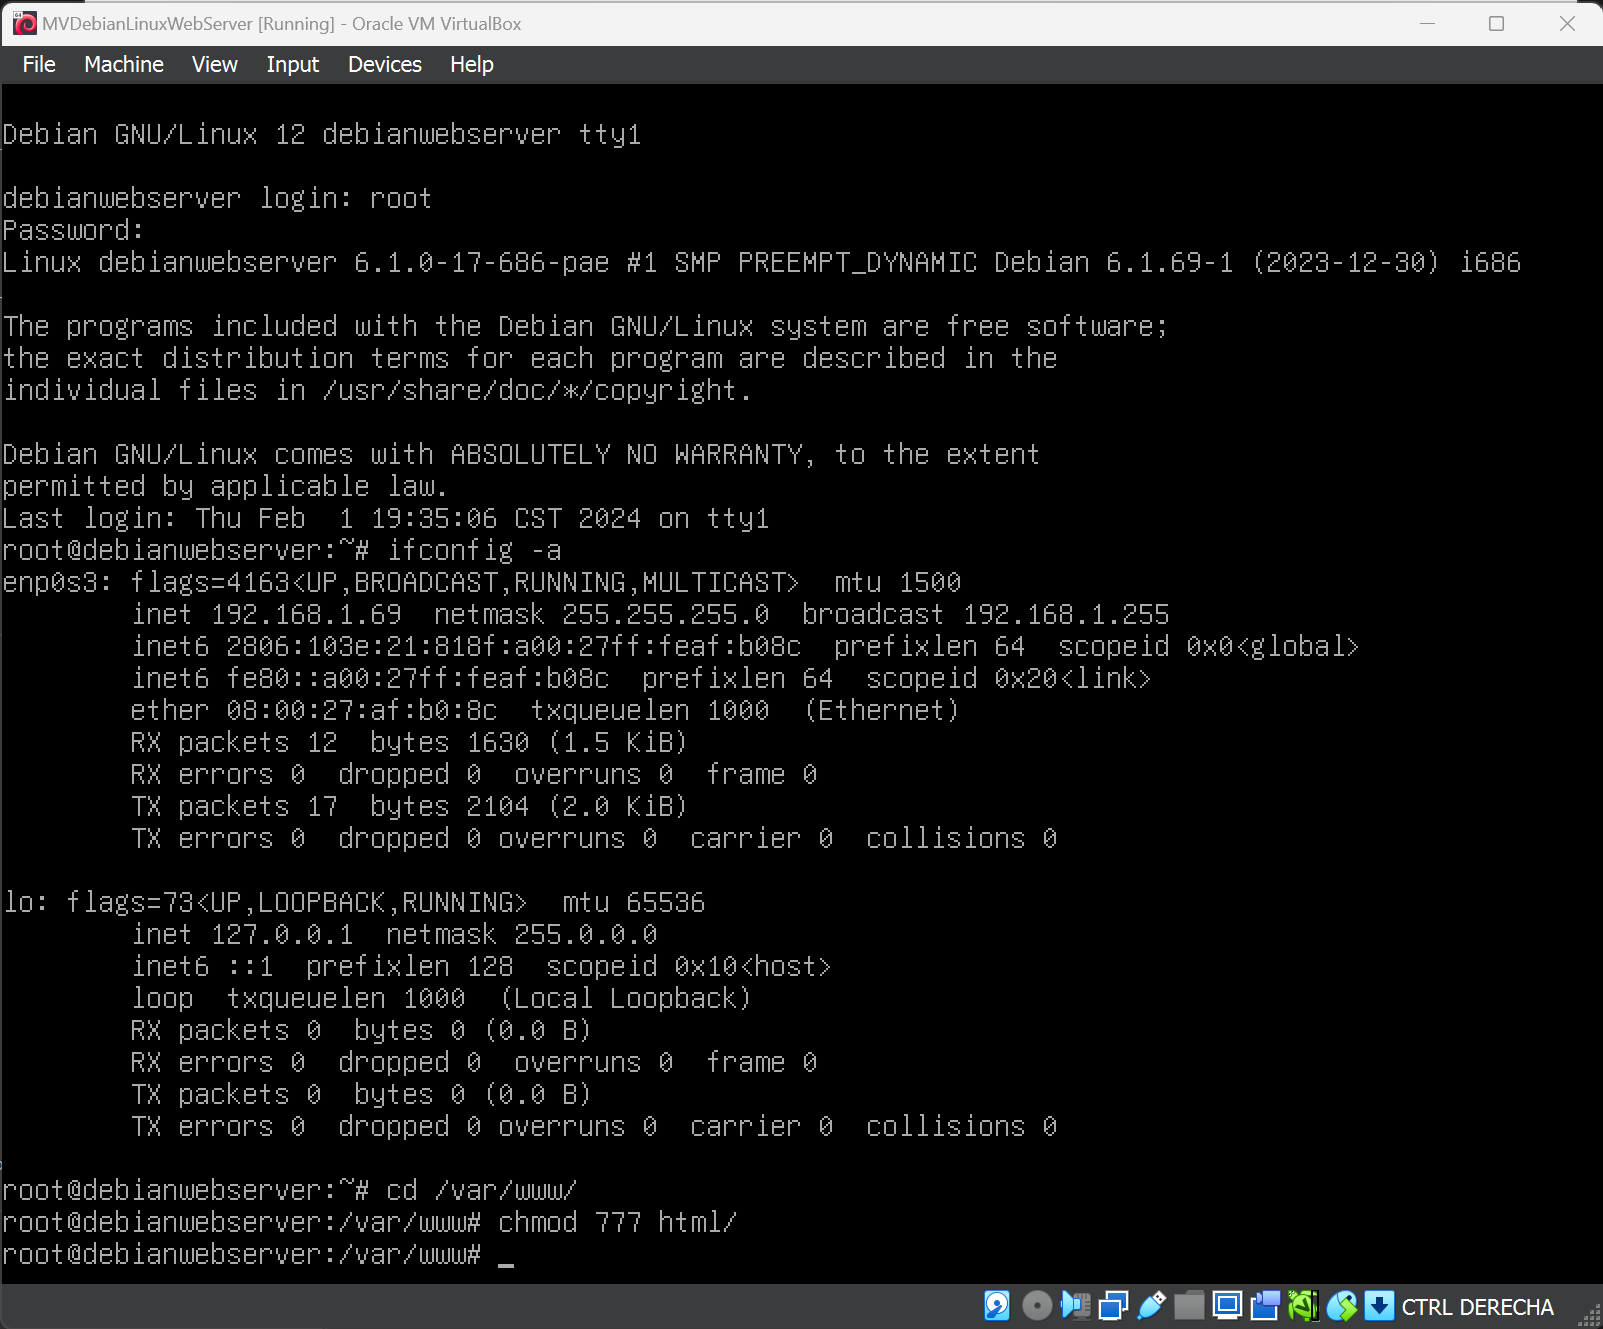
\includegraphics[width=1\linewidth]{M3_Virtualización_y_Contenedores/Tarea_2_Máquina_Virtual_Local/reporte/figuras/6-2_Carga_Sitio_Web_en_MV.png}
    \captionof{lstlisting}{Cargado de sitio web en la Máquina Virtual}
    \label{fig:Cargado_sitio_web_2}
\end{figure}


\section{Descripción de los resultados obtenidos}

A través de la IP que se obtiene ejecutando el comando \textbf{ifconfig} abrimos un explorador web y procedemos a ingresar la IP para visualizar si se carga la página web y estamos accediendo a nuestro pequeño servidor en la máquina virtual, como se puede ver en la figura \ref{fig:Resultados_1} la página carga de forma correcta, incluso procedemos a interactuar con la misma para poder ver determinar si la interacción con la misma funciona de forma correcta como se muestra en la figura \ref{fig:Resultados_2}. En este caso es exitoso el resultado obtenido, no se presentan problemas con la renderización de la página web, ni con la interacción con la misma.

\begin{figure}[H]
    \centering
    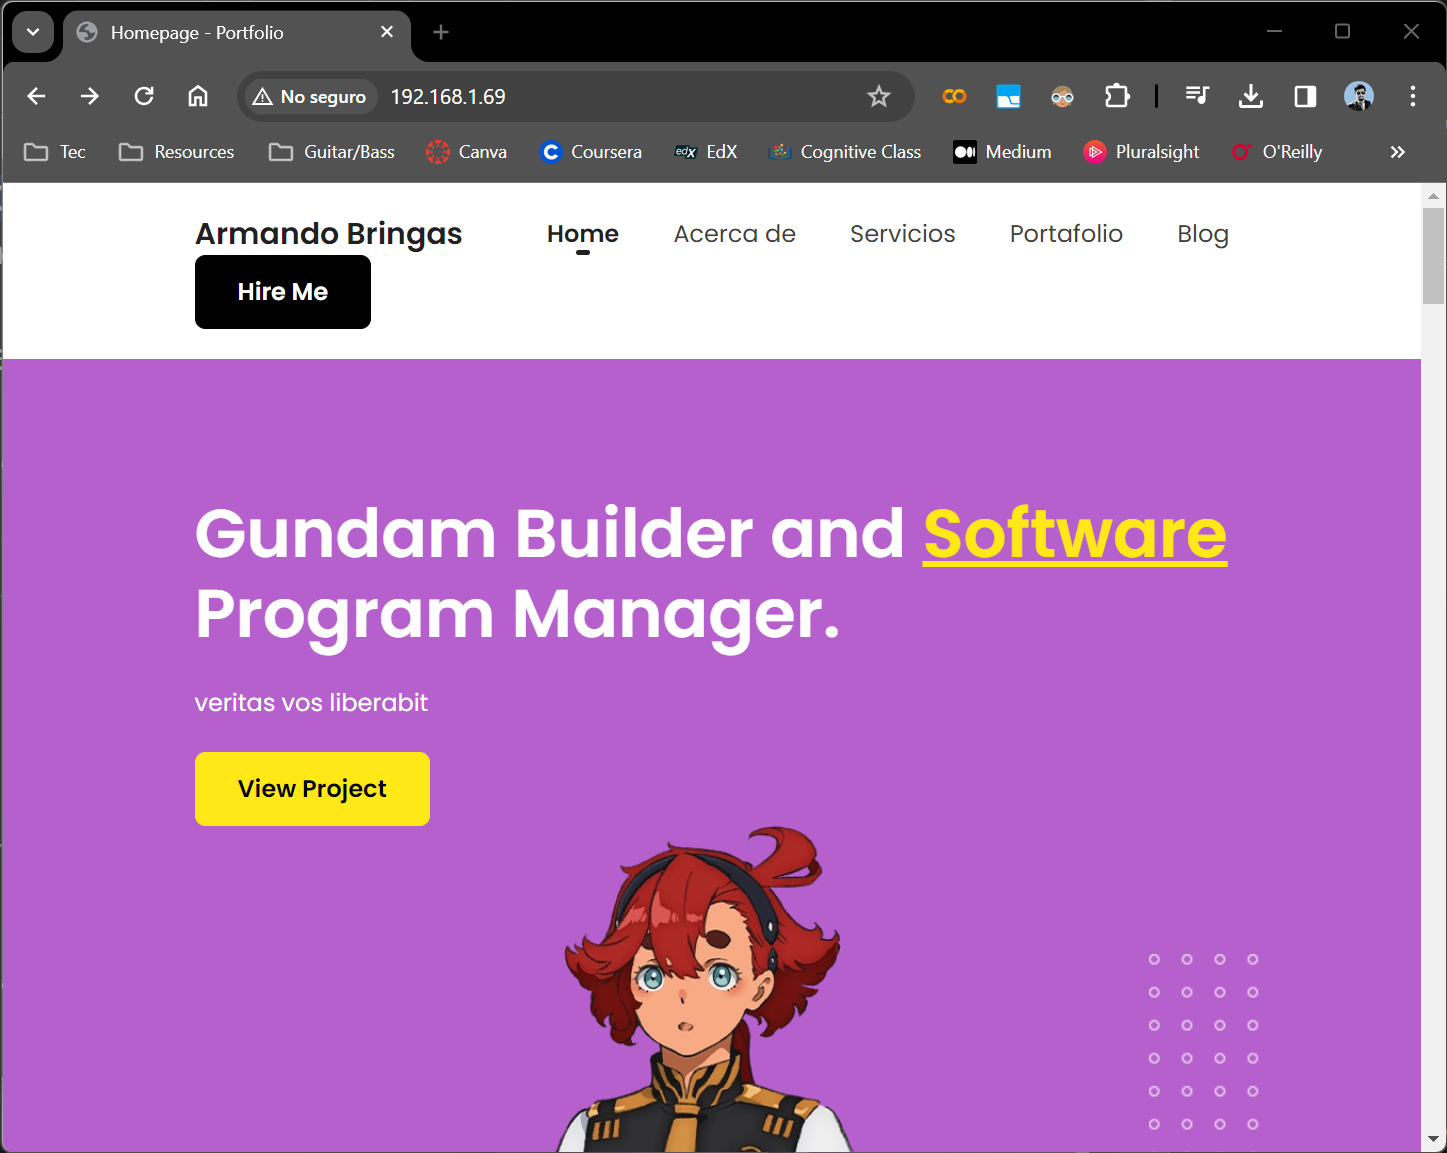
\includegraphics[width=.75\linewidth]{M3_Virtualización_y_Contenedores/Tarea_2_Máquina_Virtual_Local/reporte/figuras/7-1_Resultados.png}
    \captionof{lstlisting}{Resultados obtenidos}
    \label{fig:Resultados_1}
\end{figure}


\begin{figure}[H]
    \centering
    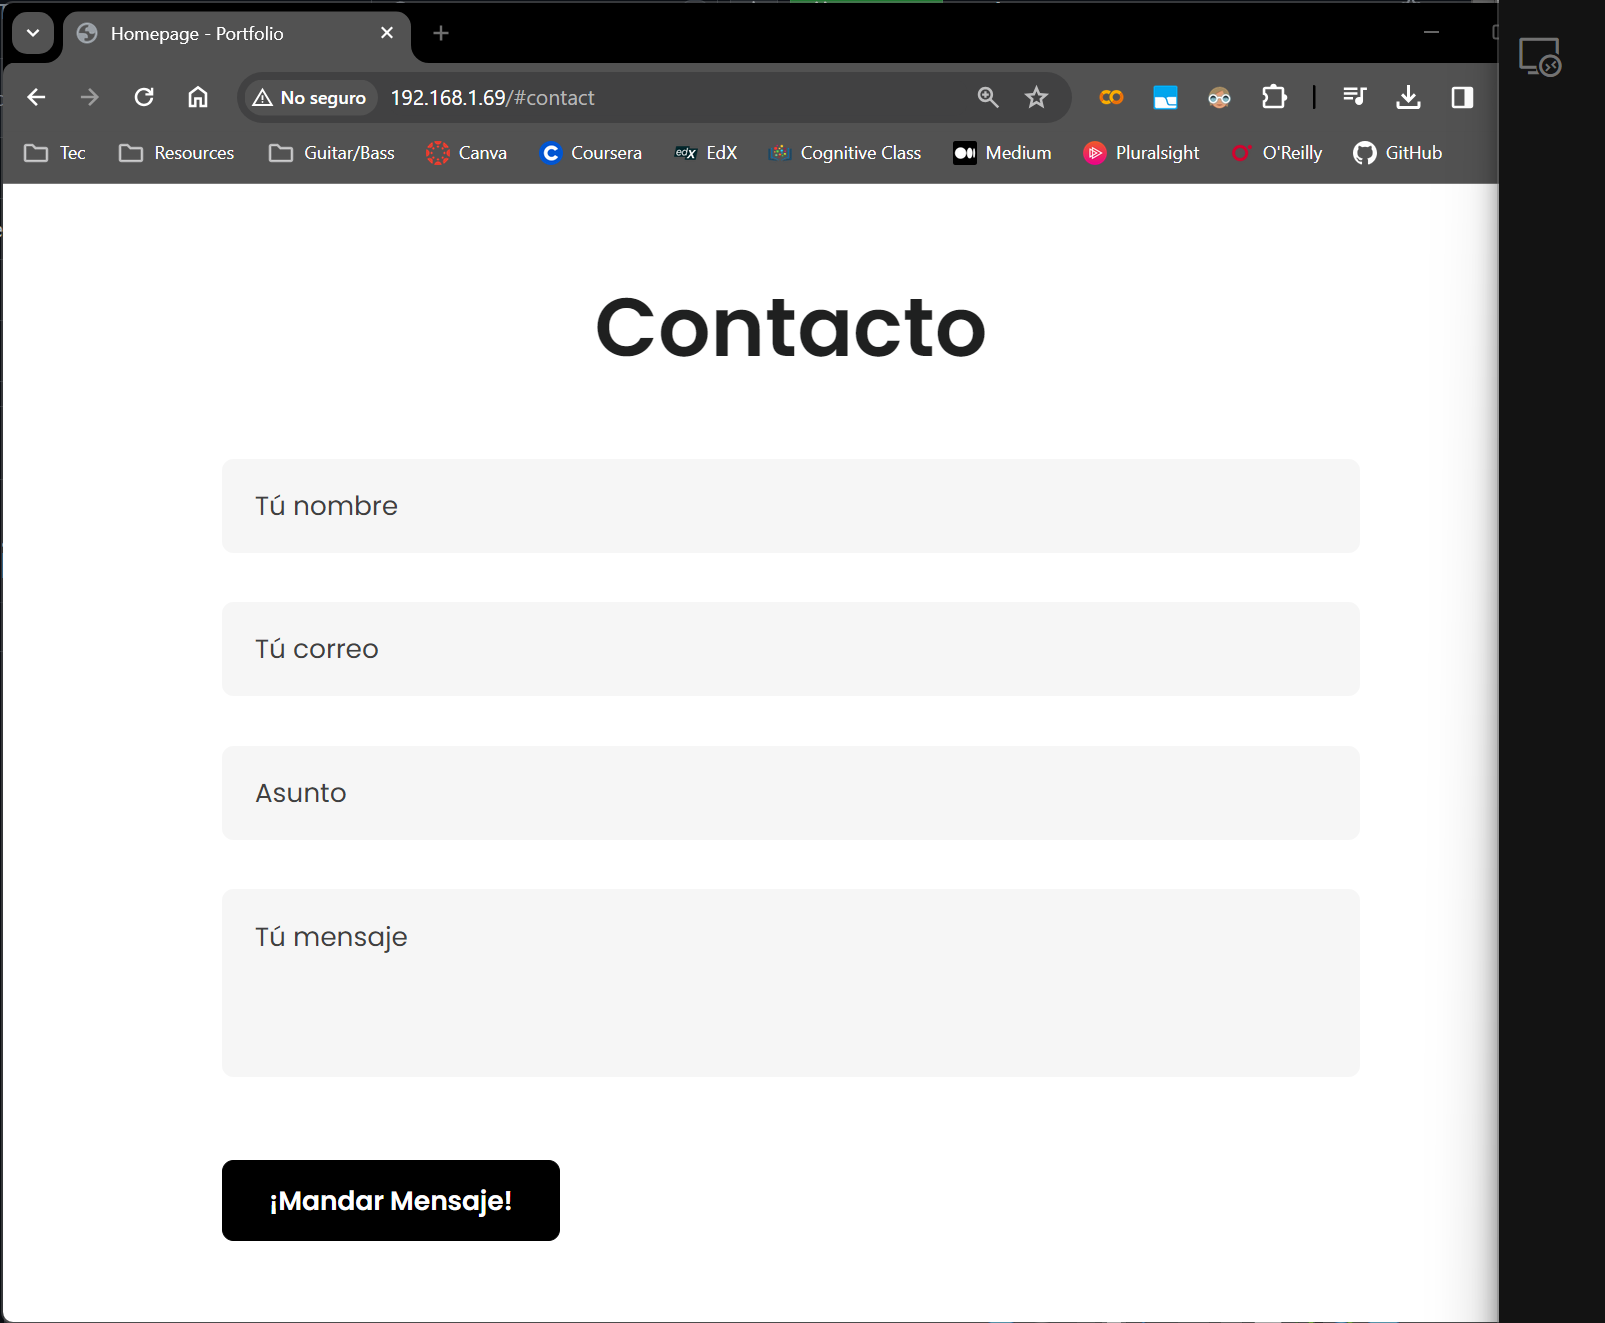
\includegraphics[width=.75\linewidth]{M3_Virtualización_y_Contenedores/Tarea_2_Máquina_Virtual_Local/reporte/figuras/7-2_Resultados.png}
    \captionof{lstlisting}{Resultados obtenidos}
    \label{fig:Resultados_2}
\end{figure}


\section{Reflexión sobre las Máquinas Virtuales}

Como pudimos experimentar con la práctica pudimos experimentar con uno de los servicios más básicos con los que comenzó el cómputo en la nube que nos da como principal ventaja el simular diferentes entornos en un mismo equipo, como pueden ser diferentes sistemas operativos. 

\vspace{1em}

Vemos como ventaja que la virtualización de diferentes entornos nos permite experimentar con diferentes sistemas operativos sin tener que hacer una partición de nuestro disco duro de la computadora y hacer configuraciones un tanto tediosas para poder por ejemplo desde el BIOS ejecutar dos sistemas operativos a la vez, también observamos que a través de la virtualización nos dejamos relativamente de preocupar por configurar drivers y la capacidad de asignar los recursos que queramos destinar nuestra Máquina Virtual.

\vspace{1em}

Ahora bien, una de las desventajas que observamos es que el uso de Máquinas Virtuales con el proceso que realizamos ya no se adapte a las prácticas actuales de Cómputo en la Nube, los recursos están limitados a la capacidad de nuestra computadora y en una última instancia nos puede resultar más conveniente el contratar un servicio IaaS a través de algún proveedor donde no nos tengamos que preocupar por ir expandiendo horizontal y verticalmente nuestros recursos y la capacidad de los mismos.

\vspace{1em}

Por último, con anterioridad ya habíamos tenido oportunidad de emplear Máquinas Virtuales, en este caso para la emulación de videojuegos en donde se han generado diferentes distribuciones basadas en Linux para poder ejecutar emuladores de diferentes sistemas de videojuegos, lo cual resulta muy práctico en muchos casos sencillo ya que también hay una comunidad detrás que se ha encargado de optimizar estos sistemas.

\vspace{1em}

Sin embargo, en alguna ocasión tratamos de utilizar una Máquina Virtual para poder ejecutar Tensorflow (un paquete de Deep Learning) cuya instalación es más sencilla en Linux, ya que su última versión ya no es de forma nativa compatible con Windows, en este caso no fue exitosa nuestra instalación ya que no encontramos la manera de configurar la tarjeta gráfica (GPU) para su utilización. Por el contrario, nos fue más práctico el utilizar WSL el cual es un subsistema de de Windows que nos permitió la instalación de Linux, y al momento de instalar TensorFlow en el mismo pudimos configurar exitosamente la tarjeta gráfica.


\vspace{1em}

\end{document}